\documentclass{ximera}
\graphicspath{  %% When looking for images,
{./}            %% look here first,
{./pictures/}   %% then look for a pictures folder,
{../pictures/}  %% which may be a directory up.
{../../pictures/}  %% which may be a directory up.
{../../../pictures/}  %% which may be a directory up.
{../../../../pictures/}  %% which may be a directory up.
}

\usepackage{listings}
\usepackage{circuitikz}
\usepackage{xcolor}
\usepackage{amsmath,amsthm}
\usepackage{subcaption}
\usepackage{graphicx}
\usepackage{tikz}
\usepackage{tikz-3dplot}
\usepackage{amsfonts}
\usepackage{mdframed} % For framing content
\usepackage{tikz-cd}

  \renewcommand{\vector}[1]{\left\langle #1\right\rangle}
  \newcommand{\arrowvec}[1]{{\overset{\rightharpoonup}{#1}}}
  \newcommand{\ro}{\texttt{R}}%% row operation
  \newcommand{\dotp}{\bullet}%% dot product
  \renewcommand{\l}{\ell}
  \let\defaultAnswerFormat\answerFormatBoxed
  \usetikzlibrary{calc,bending}
  \tikzset{>=stealth}
  




%make a maroon color
\definecolor{maroon}{RGB}{128,0,0}
%make a dark blue color
\definecolor{darkblue}{RGB}{0,0,139}
%define the color fourier0 to be the maroon color
\definecolor{fourier0}{RGB}{128,0,0}
%define the color fourier1 to be the dark blue color
\definecolor{fourier1}{RGB}{0,0,139}
%define the color fourier 1t to be the light blue color
\definecolor{fourier1t}{RGB}{173,216,230}
%define the color fourier2 to be the dark green color
\definecolor{fourier2}{RGB}{0,100,0}
%define teh color fourier2t to be the light green color
\definecolor{fourier2t}{RGB}{144,238,144}
%define the color fourier3 to be the dark purple color
\definecolor{fourier3}{RGB}{128,0,128}
%define the color fourier3t to be the light purple color
\definecolor{fourier3t}{RGB}{221,160,221}
%define the color fourier0t to be the red color
\definecolor{fourier0t}{RGB}{255,0,0}
%define the color fourier4 to be the orange color
\definecolor{fourier4}{RGB}{255,165,0}
%define the color fourier4t to be the darker orange color
\definecolor{fourier4t}{RGB}{255,215,0}
%define the color fourier5 to be the yellow color
\definecolor{fourier5}{RGB}{255,255,0}
%define the color fourier5t to be the darker yellow color
\definecolor{fourier5t}{RGB}{255,255,100}
%define the color fourier6 to be the green color
\definecolor{fourier6}{RGB}{0,128,0}
%define the color fourier6t to be the darker green color
\definecolor{fourier6t}{RGB}{0,255,0}

%New commands for this doc for errors in copying
\newcommand{\eigenvar}{\lambda}
%\newcommand{\vect}[1]{\mathbf{#1}}
\renewcommand{\th}{^{\text{th}}}
\newcommand{\st}{^{\text{st}}}
\newcommand{\nd}{^{\text{nd}}}
\newcommand{\rd}{^{\text{rd}}}
\newcommand{\paren}[1]{\left(#1\right)}
\newcommand{\abs}[1]{\left|#1\right|}
\newcommand{\R}{\mathbb{R}}
\newcommand{\C}{\mathbb{C}}
\newcommand{\Hilb}{\mathbb{H}}
\newcommand{\qq}[1]{\text{#1}}
\newcommand{\Z}{\mathbb{Z}}
\newcommand{\N}{\mathbb{N}}
\newcommand{\q}[1]{\text{``#1''}}
%\newcommand{\mat}[1]{\begin{bmatrix}#1\end{bmatrix}}
\newcommand{\rref}{\text{reduced row echelon form}}
\newcommand{\ef}{\text{echelon form}}
\newcommand{\ohm}{\Omega}
\newcommand{\volt}{\text{V}}
\newcommand{\amp}{\text{A}}
\newcommand{\Seq}{\textbf{Seq}}
\newcommand{\Poly}{\textbf{P}}
\renewcommand{\quad}{\text{    }}
\newcommand{\roweq}{\simeq}
\newcommand{\rowop}{\simeq}
\newcommand{\rowswap}{\leftrightarrow}
\newcommand{\Mat}{\textbf{M}}
\newcommand{\Func}{\textbf{Func}}
\newcommand{\Hw}{\textbf{Hamming weight}}
\newcommand{\Hd}{\textbf{Hamming distance}}
\newcommand{\rank}{\text{rank}}
\newcommand{\longvect}[1]{\overrightarrow{#1}}
% Define the circled command
\newcommand{\circled}[1]{%
  \tikz[baseline=(char.base)]{
    \node[shape=circle,draw,inner sep=2pt,red,fill=red!20,text=black] (char) {#1};}%
}

% Define custom command \strikeh that just puts red text on the 2nd argument
\newcommand{\strikeh}[2]{\textcolor{red}{#2}}

% Define custom command \strikev that just puts red text on the 2nd argument
\newcommand{\strikev}[2]{\textcolor{red}{#2}}

%more new commands for this doc for errors in copying
\newcommand{\SI}{\text{SI}}
\newcommand{\kg}{\text{kg}}
\newcommand{\m}{\text{m}}
\newcommand{\s}{\text{s}}
\newcommand{\norm}[1]{\left\|#1\right\|}
\newcommand{\col}{\text{col}}
\newcommand{\sspan}{\text{span}}
\newcommand{\proj}{\text{proj}}
\newcommand{\set}[1]{\left\{#1\right\}}
\newcommand{\degC}{^\circ\text{C}}
\newcommand{\centroid}[1]{\overline{#1}}
\newcommand{\dotprod}{\boldsymbol{\cdot}}
%\newcommand{\coord}[1]{\begin{bmatrix}#1\end{bmatrix}}
\newcommand{\iprod}[1]{\langle #1 \rangle}
\newcommand{\adjoint}{^{*}}
\newcommand{\conjugate}[1]{\overline{#1}}
\newcommand{\eigenvarA}{\lambda}
\newcommand{\eigenvarB}{\mu}
\newcommand{\orth}{\perp}
\newcommand{\bigbracket}[1]{\left[#1\right]}
\newcommand{\textiff}{\text{ if and only if }}
\newcommand{\adj}{\text{adj}}
\newcommand{\ijth}{\emph{ij}^\text{th}}
\newcommand{\minor}[2]{M_{#2}}
\newcommand{\cofactor}{\text{C}}
\newcommand{\shift}{\textbf{shift}}
\newcommand{\startmat}[1]{
  \left[\begin{array}{#1}
}
\newcommand{\stopmat}{\end{array}\right]}
%a command to give a name to explorations and hints and theorems
\newcommand{\name}[1]{\begin{centering}\textbf{#1}\end{centering}}
\newcommand{\vect}[1]{\vec{#1}}
\newcommand{\dfn}[1]{\textbf{#1}}
\newcommand{\transpose}{\mathsf{T}}
\newcommand{\mtlb}[2][black]{\texttt{\textcolor{#1}{#2}}}
\newcommand{\RR}{\mathbb{R}} % Real numbers
\newcommand{\id}{\text{id}}

\author{Zack Reed} %PEter Selinger
\title{Review and Geometry of 2D and 3D Systems of Equations}
\begin{document}
\begin{abstract}
Here we introduce one of the most prevalent applications of matrices and vectors, the solving of systems of equations.
\end{abstract}
\maketitle
    
    %\end{onlineOnly}
     
    \begin{exploration}\name{Review: Possible Outcomes of 2x2 and 3x2 Systems}
    
      Here's a brief review of the possible outcomes of 2x2 and 3x2 systems of equations.
       
      Given a system of two equations with two unknowns, there are three possible geometric outcomes. 
      
      \begin{itemize}
          \item First, the graphs of the two equations intersect at a point.  If this is the case, the system has exactly one solution. We say that the system is \dfn{consistent} and has a \dfn{unique solution}. 
           
          \begin{center}
            \begin{tikzpicture}
             
              \draw[<->] (-4,0)--(4,0);
              \draw[<->] (0,-4)--(0,4);
             
             \draw[line width=1pt](-4, -3)--(4,2);
             \draw[line width=1pt](3, -4)--(1,4);
                 
            \end{tikzpicture}
            \end{center}
          \item Second, the two lines may have no points in common.  If this is the case, the system has no solutions.  We say that the system is \dfn{inconsistent}. 
          \begin{center}
            \begin{tikzpicture}
             
              \draw[<->] (-4,0)--(4,0);
              \draw[<->] (0,-4)--(0,4);
             
             \draw[line width=1pt](-4, -4)--(4,1);
             \draw[line width=1pt](-4, -2)--(4,3);
                 
            \end{tikzpicture}
            \end{center}
          \item Finally, the two lines may coincide.  In this case, there are infinitely many points that satisfy both equations simultaneously.  We say that the system is consistent and has infinitely many solutions.
          \begin{center}
          \begin{tikzpicture}
           
            \draw[<->] (-4,0)--(4,0);
            \draw[<->] (0,-4)--(0,4);
           
           \draw[line width=2pt](-4, -3)--(4,2);
            
               
          \end{tikzpicture}
          \end{center}
          \end{itemize}
      
                  Given a linear system in two variables and more than two equations, we have a variety of geometric possibilities.  In terms of the number of solutions, there are three possibilities.
       
                  \begin{itemize}
                  \item First, it is possible for the graphs of all equations in the system to intersect at a single point, giving us a unique solution. 
                   
                  \begin{center}
                  \begin{tikzpicture}
                   
                    \draw[<->] (-4,0)--(4,0);
                    \draw[<->] (0,-4)--(0,4);
                   
                   \draw[line width=1pt](-2, 4)--(4,1);
                   \draw[line width=1pt](3, 4)--(-1,-4);
                   \draw[line width=1pt](1, 4)--(4,-2);
                       
                  \end{tikzpicture}
                  \end{center}
                   
                  \item Second, it is possible for the graphs to have no points common to all of them.  If this is the case, the system is inconsistent.
                   
                  %\begin{center}[3in]
                  \begin{center}
                  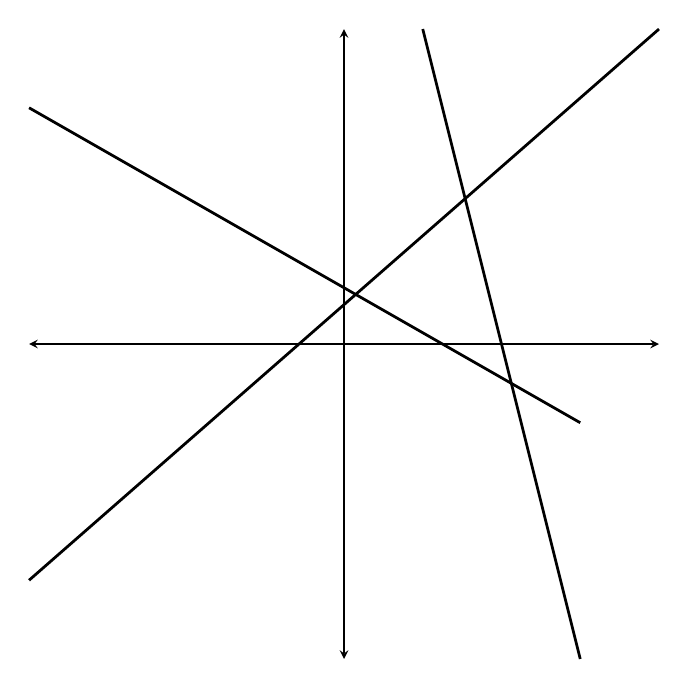
\begin{tikzpicture}
                   
                    \draw[<->] (-4,0)--(4,0);
                    \draw[<->] (0,-4)--(0,4);
                   
                   \draw[line width=1pt](-4, -3)--(4,4);
                   \draw[line width=1pt](3, -4)--(1,4);
                   \draw[line width=1pt](3, -1)--(-4,3);
                       
                  \end{tikzpicture}\quad\quad
                  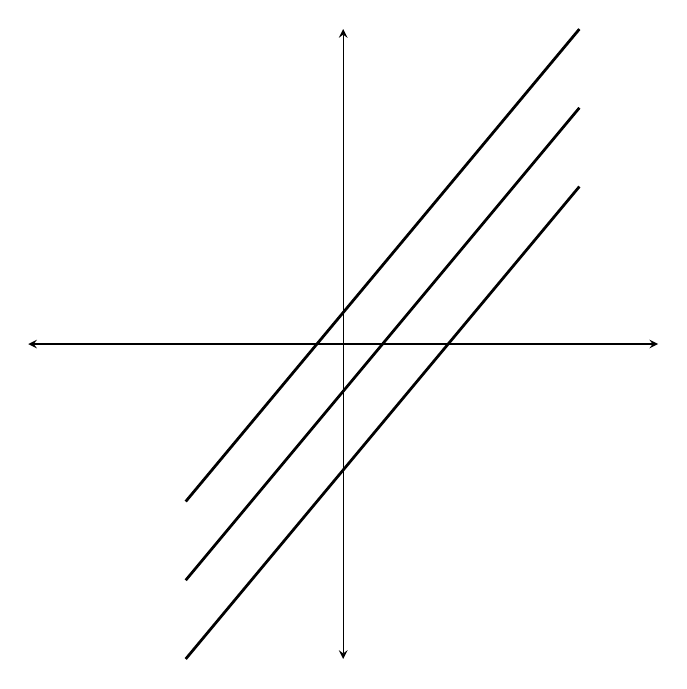
\begin{tikzpicture}
                   
                    \draw[<->] (-4,0)--(4,0);
                    \draw[<->] (0,-4)--(0,4);
                   
                   \draw[line width=1pt](-2, -3)--(3,3);
                   \draw[line width=1pt](-2, -2)--(3,4);
                   \draw[line width=1pt](-2, -4)--(3,2);
                       
                  \end{tikzpicture}
                  \end{center}
                  %\end{center}
                   
                  \item Finally, it is possible for all of the lines to coincide, giving us infinitely many solutions.
                  \end{itemize}
  
    \end{exploration}
    
  \begin{exploration}\name{Geometry of Linear Systems in Three Variables}
    Let's now consider the following  system of three equations and three unknowns

    $$\begin{array}{ccccccc}
        3x & -&y&+&z&= &0 \\
        2x& +&y&+&2z&=&2\\
        x& +&4y&-&2z&=&11.
    \end{array}$$

    Introducing a third variable means that each equation describes a plane in $\mathbb{R}^3$, rather than a line in $\mathbb{R}^2$.  Luckily, we again preserve the solution set by the same row operations, so our strategy for solving systems of equations remains the same.

    \begin{example}

        Use the GeoGebra environment to solve the system of equations above. 

        \geogebra{stvqh3ts}{1219}{521}

        \begin{hint}

            The solution to the system is $(1,2,-1)$, as depicted in the GeoGebra environment. If your constant terms are different, you may have made a mistake in your row operations.

        \end{hint}

        \begin{solution}

            The system can be solved by the following row operations (you may first need to swap rows to get the order to match the stated system above):

            %I NEED TO COME BACK AND JUST DO FRACTIONs

            $$R_2\rightarrow R_2-2R_3$$

            $$R_1\rightarrow R_1-3R_3$$

            $$R_2\rightarrow -R_2/7$$

            $$R_1\rightarrow R_1+13R_2$$

            $$R_3\rightarrow R_3-4R_2$$

            $$R_1\rightarrow -R_1/4.14$$

            $$R_2\rightarrow R_2+.86R_1$$

            $$R_3\rightarrow R_3-1.43R_1$$

            $$R_1\leftrightarrow R_3$$

            This gives the system 

            $$\begin{array}{ccccccc}
                 1x& +0y&+0z &=&1 \\
                0x&+1y& +0z& =&2\\
                0x &+1y &+1z 1z&=&-1.
            \end{array}$$

        \end{solution}
    \end{example}

    \begin{remark}

        Notice that the final system visualized as entirely horizontal or vertical planes, corresponding to the equations $x=1$, $y=2$, and $z=-1$. This reduction to standard planes has an important corrolary in the next section, where we examine row operations from the perspective of matrices. 

    \end{remark}

    Now, let's use row operations to determine the geometry of less nice systems.

\begin{example}

    Use the GeoGebra environment to analyze the following system of equations, which again creates the third equation from the first two via linear combination:

    $$\begin{array}{ccccccc}
        2x & +&3y&-&z&= &5 \\
        x& -&y&+&4z&=&6\\
        4x& +&y&+&7z&=&17.
    \end{array}$$

    As always, use row operations to solve the system. We're going to pay particular attention to the format of the "solved" system at the end of this section, and in the coming sections as well.

    \begin{solution}

        While you don't need to know this to solve the system using row operations, the third row is created from $R_1+2*R_2$. So, again, the geometric reason that we don't have a solution is that the first two planes intersect at a line (rather than a point) and then the third plane doesn't change the solution set of the system, and hence does not create a new intersection point.

        Solving the system using row operations (without the knowledge above) can be done in steps simlar to the following:

        $$R_3\rightarrow R_3-4R_2$$

        $$R_1\rightarrow R_1-2R_2$$

        At this stage, note that $R_1$ and $R_3$ are the exact same equations, and so we can get rid of one by subtracting the other.

        $$R_1\rightarrow R_1-R_3$$

        Now, we see just the two "spanning" planes of the system, and can further reduce them as much as possible, but not likely to standard vertical or horizontal planes.

        $$R_3\rightarrow R_3/5$$

        $$R_2\rightarrow R_2+R_3$$

        $$R_1\rightleftarrows R_2$$

        $$R_2\rightleftarrows R_3$$

        This gives the system, in its most reduced form:

        $$\begin{array}{ccccccc}
            1x& +0y&+2.2z &=&4.6 \\
            0x&+1y& -1.8z& =&-1.4\\
            0x &+0y &+0z &=&0.
        \end{array}$$

        So, here, we again have infinitely many solutions, as any point along the intersecting line between the two planes will satisfy the system.

        In this case, let's set $z=\tau$, which is an unknown constant value. This changes the system to be 

        $$\begin{array}{ccccccc}
            1x& +0y&+2.2\tau &=&4.6 \\
            0x&+1y& -1.8\tau& =&-1.4\\
            0x &+0y &+0\tau &=&0.
        \end{array}$$

        Note that the third equations is still true for any number $\tau$. Then since $\tau$ is just some unknown constant, we can solve for $x$ and $y$, getting

        $$x=4.6-2.2\tau$$
        
        $$y=-1.4+1.8\tau.$$

        So any points of the form $(4.6-2.2\tau, -1.4+1.8\tau, \tau)$ will satisfy the system.

    \end{solution}

\end{example}

\end{exploration}

\begin{exploration}\name{Review: Possible Outcomes of 3x3 Systems}

We'll be unpacking more examples of systems with or without solutions in the homework, but here's an overview of the different ways that solutions can or can't exist for 3x3 systems of equations.

Given a linear system of three equations in three variables, there are three ways in which the system can be consistent.

\begin{itemize}
    \item First, the three planes could intersect at a single point, giving us a unique solution.
    \begin{center}
        \tdplotsetmaincoords{70}{130}
            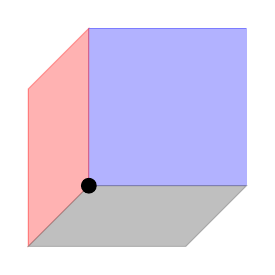
\begin{tikzpicture}
        \filldraw[blue, opacity=0.3](0,0,0)--(2,0,0)--(2,2,0)--(0,2,0)--cycle;
        \filldraw[red, opacity=0.3] (0,0,0)--(0,0,2)--(0,2,2)--(0,2,0)--cycle;
        \filldraw[gray, opacity=0.5] (0,0,0)--(0,0,2)--(2,0,2)--(2,0,0)--cycle;
        \fill[] (0,0,0) circle (0.1cm);
            \end{tikzpicture}
        \end{center}
    \item Second, the three planes can intersect in a line, forming a paddle-wheel shape.  In this case, every point along the line of intersection is a solution to the system, giving us infinitely many solutions.
        \begin{center}
        \tdplotsetmaincoords{70}{130}
                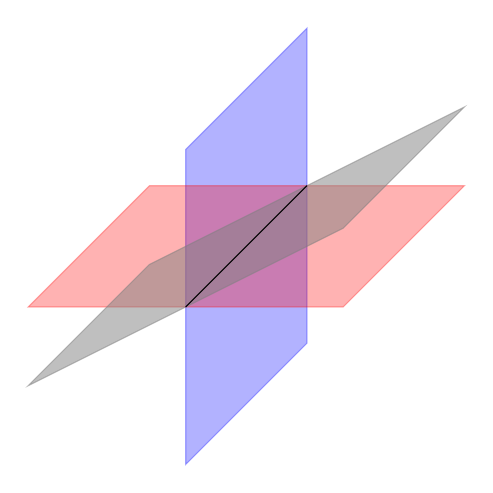
\begin{tikzpicture}
                \filldraw[blue, opacity=0.3](0,-2,2)--(0,2,2)--(0,2,-2)--(0,-2,-2)--cycle;
                \filldraw[red, opacity=0.3] (2,0,2)--(-2,0,2)--(-2,0,-2)--(2,0,-2)--cycle;
                \filldraw[gray, opacity=0.5] (2,1,2)--(2,1,-2)--(-2,-1,-2)--(-2,-1,2)--cycle;
                \draw[-](0,0,-2)--(0,0,2) ;
            \end{tikzpicture}
            \end{center}
    \item Finally, the three planes can coincide.  If this is the case, there are infinitely many solutions.
        \begin{center}
        \tdplotsetmaincoords{70}{130}
            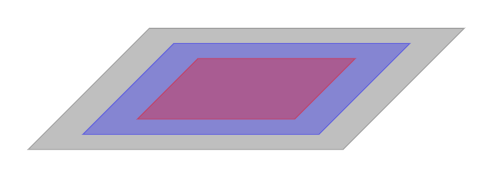
\begin{tikzpicture}
                \filldraw[gray, opacity=0.5] (2,0,2)--(-2,0,2)--(-2,0,-2)--(2,0,-2)--cycle;
                \filldraw[blue, opacity=0.3] (1.5,0,1.5)--(-1.5,0,1.5)--(-1.5,0,-1.5)--(1.5,0,-1.5)--cycle;
                \filldraw[red, opacity=0.3] (1,0,1)--(-1,0,1)--(-1,0,-1)--(1,0,-1)--cycle;
            \end{tikzpicture}
        \end{center}
\end{itemize}

There are four ways for a system to be inconsistent.  They are depicted below.
%\begin{center}[4in]
\begin{center}
\tdplotsetmaincoords{70}{130}
    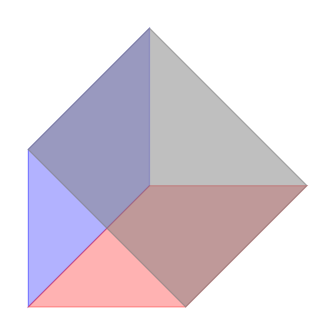
\begin{tikzpicture}
        \filldraw[blue, opacity=0.3](0,0,2)--(0,2,2)--(0,2,-2)--(0,0,-2)--cycle;
        \filldraw[red, opacity=0.3] (2,0,2)--(0,0,2)--(0,0,-2)--(2,0,-2)--cycle;
        \filldraw[gray, opacity=0.5] (0,2,2)--(0,2,-2)--(2,0,-2)--(2,0,2)--cycle;
    \end{tikzpicture}\quad
    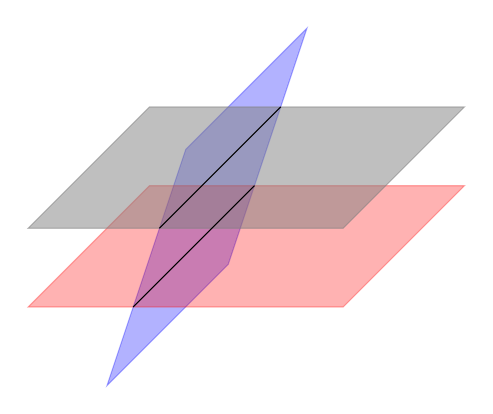
\begin{tikzpicture}
        \filldraw[blue, opacity=0.3](-1,-1,2)--(0,2,2)--(0,2,-2)--(-1,-1,-2)--cycle;
        \filldraw[red, opacity=0.3] (2,0,2)--(-2,0,2)--(-2,0,-2)--(2,0,-2)--cycle;
        \filldraw[gray, opacity=0.5] (2,1,2)--(-2,1,2)--(-2,1,-2)--(2,1,-2)--cycle;
        \draw[-](-2/3,0,-2)--(-2/3,0,2) ;
        \draw[-](-1/3,1,-2)--(-1/3,1,2) ;
    \end{tikzpicture}\quad
    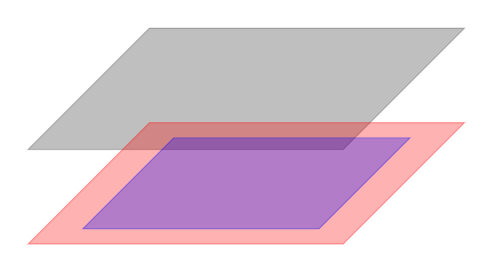
\begin{tikzpicture}
        \filldraw[gray, opacity=0.5] (2,1.2,2)--(-2,1.2,2)--(-2,1.2,-2)--(2,1.2,-2)--cycle;
        \filldraw[red, opacity=0.3] (2,0,2)--(-2,0,2)--(-2,0,-2)--(2,0,-2)--cycle;
        \filldraw[blue, opacity=0.3] (-1.5,0,1.5)--(-1.5,0,-1.5)--(1.5,0,-1.5)--(1.5,0,1.5)--cycle;
    \end{tikzpicture}\quad
    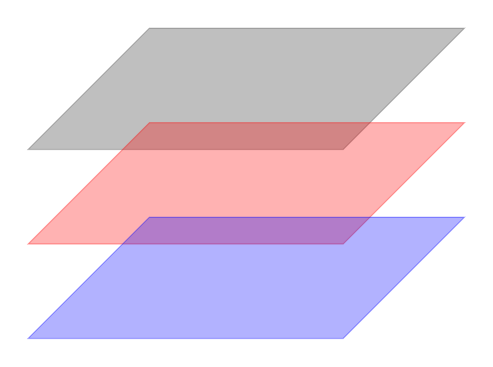
\begin{tikzpicture}
        \filldraw[gray, opacity=0.5] (2,1.2,2)--(-2,1.2,2)--(-2,1.2,-2)--(2,1.2,-2)--cycle;
        \filldraw[red, opacity=0.3] (2,0,2)--(-2,0,2)--(-2,0,-2)--(2,0,-2)--cycle;
        \filldraw[blue, opacity=0.3] (2,-1.2,2)--(-2,-1.2,2)--(-2,-1.2,-2)--(2,-1.2,-2)--cycle;
    \end{tikzpicture}
\end{center}

\end{exploration}

In the next chapter, we'll apply these ideas to the notion of matrix inverses, which take a much more intentional orientation towards interpreting these operations for matrices, and determining whether the matrix equation 

$$A\vec{x}=\vec{b}$$

can be solved by finding an inverse matrix $A^{-1}$ that satisfies

$$\vec{x}=A^{-1}A\vec{x}=A^{-1}\vec{b}$$


\end{document}